\documentclass{ee208report}

\title{Lab Report 12}

\begin{document}

\begin{CJK}{UTF8}{gbsn}
    \maketitle
\end{CJK}

\begin{multicols*}{2}

\section{Introduction}

In this lab report, we present our implementation of
SIFT\cite{lowe2004distinctive} through a combination of OpenCV's built-in
functions and techniques suggested in the paper. SIFT, short for scale invariant
feature transform, describe an image by its distinctive features in the form of
keypoints and associated feature descriptors.

The report centers around the implementation and performance of SIFT. We decompose SIFT into a series of steps in Section~\ref{s:anatomy} and explain our implementation for each step in the sections that follow.

\section{Anatomy of SIFT}
\label{s:anatomy}

SIFT involves the following steps\footnote{\underline{\href{http://aishack.in/
tutorials/sift-scale-invariant-feature-transform-introduction/}{SIFT: Theory and
Practice: Introduction - AI Shack}}}:

\begin{enumerate}
    \item \textbf{Constructing a scale space} This is the initial preparation.
    You create internal representations of the original image to ensure scale
    invariance. This is done by generating a "scale space".
    \item \textbf{LoG Approximation} The Laplacian of Gaussian is great for
    finding interesting points (or key points) in an image. But it's
    computationally expensive. So we cheat and approximate it using the
    representation created earlier.
    \item \textbf{Finding keypoints} With the super fast approximation, we now
    try to find key points. These are maxima and minima in the Difference of
    Gaussian image we calculate in step 2
    \item \textbf{Eliminate bad key points} Edges and low contrast regions are
    bad keypoints. Eliminating these makes the algorithm efficient and robust. A
    technique similar to the Harris Corner Detector is used here.
    \item \textbf{Assigning an orientation to the keypoints} An orientation is
    calculated for each key point. Any further calculations are done relative to
    this orientation. This effectively cancels out the effect of orientation,
    making it rotation invariant.
    \item \textbf{Generate SIFT features} Finally, with scale and rotation
    invariance in place, one more representation is generated. This helps
    uniquely identify features. Lets say you have 50,000 features. With this
    representation, you can easily identify the feature you're looking for
    (say, a particular eye, or a sign board).
\end{enumerate}

Due to lack of time, we didn't find keypoints with pyramids of images but used
the built-in \texttt{goodFeaturesToTrack()} to directly retrieve keypoints
instead.

\section{Implementation}

Following the outline laid out in the previous section, we present our
implementation of SIFT.

\subsection{Finding keypoints}

\texttt{goodFeaturesToTrack()} is configured to return all found keypoints:

\begin{minted}{python}
    keypoints = cv.goodFeaturesToTrack(
        img, 0, 0.01, 10).reshape(-1, 2)
\end{minted}

\subsection{Assigning orientation}

For each keypoint, a $5 \times 5$ window around the keypoint is used to find the
keypoint orientation. Since all keypoints returned by
\texttt{goodFeaturesToTrack()} have integer coordinates, no interpolation is
needed.

The magnitudes and angles of gradients that are not on the border are calculated
first.

\begin{minted}{python}
    dy = (img[2:, 1:-1].astype(np.int32)
        - img[:-2, 1:-1])
    dx = (img[1:-1, 2:].astype(np.int32)
        - img[1:-1, :-2])
    # if the image is m * n, the mags and angles
    # array are (m - 2) * (n - 2)
    mags = np.sqrt(dx * dx + dy * dy)
    angles = np.rad2deg(np.arctan2(dy, dx))
\end{minted}

\begin{figure}[H]
    \centering
    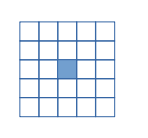
\includegraphics{images/keypoint_window.png}
    \caption{$5 \times 5$ grids for finding orientation. Each cell is a pixel.
        The cell representing the keypoint is shaded.}
    \label{fig:keypoint-window}
\end{figure}

Note that integers must be cast to an appropriate signed type before subtraction
to prevent overflow. Then, angles are converted from
$(-180^\circ, 180^\circ]$ to $[0^\circ, 360^\circ)$.

\begin{minted}{python}
    # convert angle representation from
    # (-180, 180] to [0, 360)
    angles += ((angles < 0).astype(np.int16)
        * 360)
\end{minted}

For each keypoint $(x, y)$, we calculate a histogram of angles in its $5 \times
5$ neighborhood weighted by magnitudes of gradients. Angles in the range
$[0^\circ, 360^\circ)$ are divided into 36 bins with length $10^\circ$. The bin
that collects the most weight determine the orientation. Additionally, if a bin
collects more than 80\% of the maximum weight, a keypoint with the coordinate
and the orientation of the bin is generated.

For example, if the bin $[20^\circ, 30^\circ)$ collects the most weight, the
keypoint will be assigned an orientation of $25^\circ$. If the bin $[190^\circ,
200^\circ)$ collects more than 80\% of the maximum weight, a keypoint is
generated with orientation $195^\circ$. The implementation is available in
Listing~\ref{lst:keypoint-orientation}.

\begin{figure}[H]
    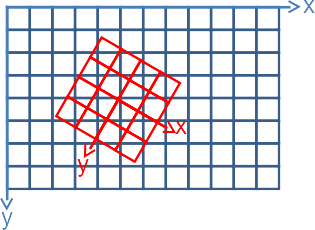
\includegraphics[width=\linewidth]{images/descriptor_grid.png}
    \caption{Demonstration of descriptor calculation. Each pixel is shown as an
        intersection. The $16 \times 16$ window is shown as a $4 \times 4$ red
        grid.}
    \label{fig:descriptor-grid}
\end{figure}

\subsection{Generate descriptors}

We calculate the descriptor over a $16 \times 16$ window. The window is tilted
in the direction of the keypoint's orientation, as shown in
Figure~\ref{fig:descriptor-grid}.

For each $4 \times 4$ window in the $16 \times 16$ window around the keypoint,
we find the coordinate of the center for each cell in the $4 \times 4$ window,
as shown in Figure~\ref{fig:descriptor-window}.

\begin{figure}[H]
    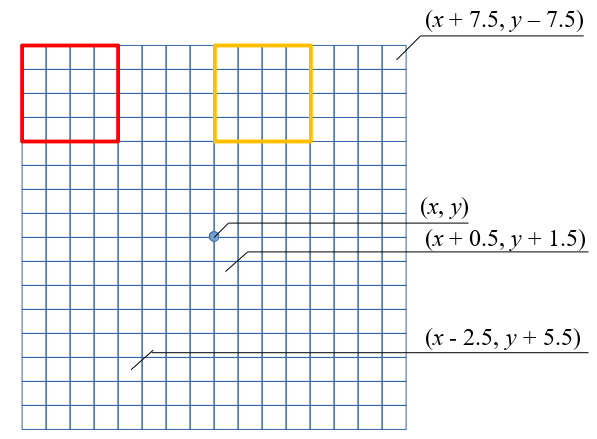
\includegraphics[width=\linewidth]{images/descriptor_window.png}
    \caption{$16 \times 16$ window for finding descriptors. Two of the total 16
        $4 \times 4$ window for finding histograms are colored yellow and gold.
        The keypoint $(x, y)$ is marked with a dark blue point. Coordinates
        (prior to rotation) are given as an example.}
    \label{fig:descriptor-window}
\end{figure}

For example, the center of the upper right cell has the coordinate $(x + 7.5, y
- 7.5)$. The $16 \times 16$ window is then rotated to match the keypoint's
orientation. Angles of gradients then are interpolated at the rotated
coordinate.

With 16 interpolated angles for each $4 \times 4$ window, a histogram is
calculated for the range $[0^\circ, 360^\circ)$ with 8 bins, i.e. an
8-dimensional vector is generated. Repeat the histogram calculation for all the
$4 \times 4$ windows to obtain 16 8-dimensional vectors. Concatenate these
vectors to form a 128-dimensional vector. This is 128-dimensional vector is the
descriptor for the keypoint.

The implementation for finding descriptors is available in Listing~\ref{lst:descriptor}.

\subsection{Keypoint matching}

To find a match in one image for a keypoint in another image, the Eculidean distance is calculated between between all descriptors in one image and the descriptor of the keypoint in another image. A match is found if and only if the ratio of minimum distance to the second minimum distance is less than 0.8.

Listing~\ref{lst:keypoint-matching} gives the code for matching keypoints and marking matched keypoints between two images.

\section{Performance}

Figure~\ref{fig:match-results} showcases the match results.

\begin{figure}[H]
    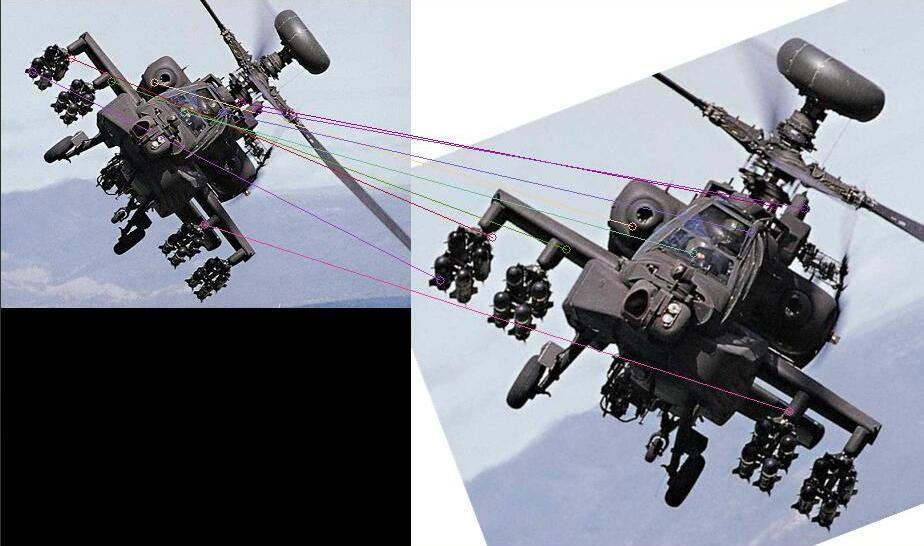
\includegraphics[width=\linewidth]{images/match_results.jpg}
    \caption{Matched keypoints}
    \label{fig:match-results}
\end{figure}

\bibliographystyle{plain}
\bibliography{lowe2004distinctive}

\end{multicols*}

\begin{listing}
    \begin{minted}[frame=lines, linenos]{python}
# find orientation for each keypoint
keypoints_with_orientation = []
for x, y in keypoints:
    x = int(x)
    y = int(y)
    # if the neighborhood sits next to the border
    if x < 3 or x + 3 > img.shape[0] or y < 3 or y + 3 > img.shape[1]:
        continue

    # draw a 5 * 5 window on magnitudes and gradients
    # Indices are offset by 1.
    mag_part = mags[y - 3: y + 2, x - 3: x + 2]
    angle_part = angles[y - 3: y + 2, x - 3: x + 2]
    histogram = np.histogram(angle_part, 36, (0, 360), weights=mag_part)[0]
    threshold = histogram.max() * 0.8
    for i, weight in enumerate(histogram):
        if weight > threshold:
            keypoints_with_orientation.append((x, y, i * 10 + 5))
    \end{minted}
    \caption{Finding an orientation for each keypoint}
    \label{lst:keypoint-orientation}
\end{listing}

\begin{listing}
    \begin{minted}[frame=lines, linenos]{python}
# generate descriptors
descriptors = []
keypoints = []
for x, y, orientation in keypoints_with_orientation:
    max_offset = 7.5 * np.sqrt(2) * np.sin((orientation / 90 + 45) / 180 * np.pi)
    # reject the keypoint if a descriptor can not be generated due to border
    if y + np.ceil(max_offset) > img.shape[0] or np.floor(y - max_offset) < 0 \
            or x + np.ceil(max_offset) > img.shape[1] or np.floor(x - max_offset) < 0:
        continue

    rad = np.deg2rad(orientation)
    rotation_matrix = np.array([
        [np.cos(rad), - np.sin(rad)], [np.sin(rad), np.cos(rad)]
    ])
    # find the rotated offsets
    rotated_offsets = np.array([[rotation_matrix @ j for j in i] for i in OFFSETS])

    descriptor = []
    # for each 4 * 4 window
    for i in range(4):
        for j in range(4):
            window = rotated_offsets[4 * i: 4 * (i + 1), 4 * j: 4 * (j + 1), :]
            # store interpolated angles
            angle_results = np.zeros((4, 4))
            # for each angle to interpolate
            for k in range(4):
                for l in range(4):
                    x_ = x + window[k][l][0]
                    y_ = y + window[k][l][1]
                    floored_x_ = np.floor(x_)
                    floored_y_ = np.floor(y_)
                    
                    dx1 = x_ - floored_x_
                    dx2 = 1 - dx1
                    dy1 = y_ - floored_y_
                    dy2 = 1 - dy1
                    
                    angle_results[k][l] = angles[y - 1][x - 1] * dx2 * dy2 \
                        + angles[y - 1][x] * dx1 * dy2 \
                        + angles[y][x - 1] * dx2 * dy1 \
                        + angles[y][x] * dx1 * dy1 \
                        - orientation
            hist = np.histogram(angle_results, 8, (0, 360))[0]
            descriptor.append(hist)
    descriptor = np.array(descriptor).reshape(128)
    norm = np.sqrt((descriptor ** 2).sum())
    if int(norm):
        descriptor = descriptor / norm
        descriptors.append(descriptor)
        keypoints.append((x, y))
    \end{minted}
    \caption{Implementation for finding descriptors}
    \label{lst:descriptor}
\end{listing}

\begin{listing}
    \begin{minted}[frame=lines, linenos]{python}
target = cv.imread('target.jpg', cv.IMREAD_GRAYSCALE)
keypoints1, descriptors1 = sift(target)
for i in range(1, 6):
    img = cv.imread('dataset/{}.jpg'.format(i), cv.IMREAD_GRAYSCALE)
    keypoints, descriptors = sift(img)
    matches_img = np.zeros((max(target.shape[0], img.shape[0]),
    target.shape[1] + img.shape[1]), np.uint8)
    matches_img[:target.shape[0], :target.shape[1]] = target
    matches_img[:img.shape[0], target.shape[1]:] = img
    n_keypoint = 0
    for j in range(keypoints1.shape[0]):
        min_distance = 4
        second_min_distance = 4
        m = -1      # index for keypoint in img with minimum distance
        for k in range(keypoints.shape[0]):
            distance = np.sqrt(((descriptors1[j] - descriptors[k]) ** 2).sum())
            print(k, distance)
            if distance < min_distance:
                second_min_distance = min_distance
                min_distance = distance
                m = k
        
        if n_keypoint > 10:
            break
        
        if min_distance / second_min_distance < 0.8:
            keypoint_in_img = (keypoints[m][0] + target.shape[0], keypoints[m][1])
            keypoint_in_target = (keypoints1[j][0], keypoints1[j][1])
            cv.circle(matches_img, keypoint_in_target, 5, 240)
            cv.circle(matches_img, keypoint_in_img, 5, 240)
            cv.line(matches_img, keypoint_in_target, keypoint_in_img, 240)
        n_keypoint += 1

    cv.imwrite('matches.png', matches_img)
    \end{minted}
    \caption{Matching keypoints}
    \label{lst:keypoint-matching}
\end{listing}

\end{document}
